\section{Content}
\begin{frame}{Objectives}
    \begin{itemize}
        \item Develop an IoT application based on technologies used so far
        \item Implement Client-Server communication between RPI and Virtualized Ubuntu
        \item RPI establishes communication with the cloud server/gateway
        \item RPI takes samples from the sensors periodically
        \item Data collected is sent to the cloud server/gateway
        \item Cloud server/gateway displays the information collected
       
    \end{itemize}
     \centering
     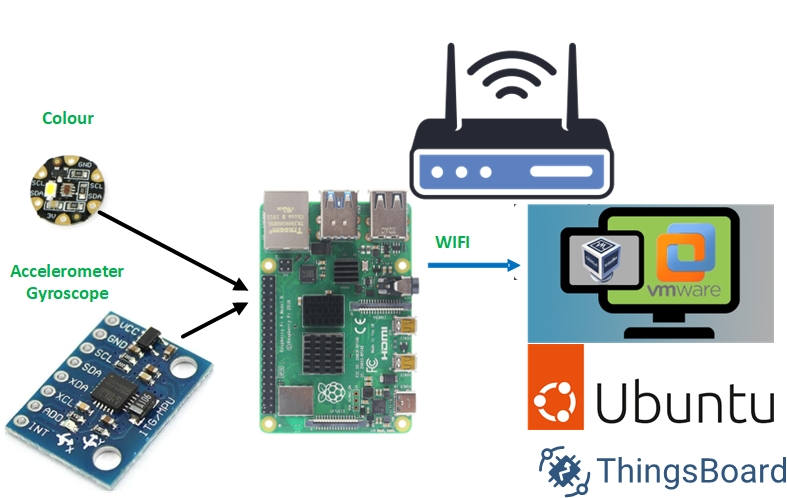
\includegraphics[width=0.5\textwidth]{trainingmaterials/project2-iot/schemacomplete.jpg}
\end{frame}

\section{Internet of Things}
\begin{frame}{Internet of Things}
    \begin{block}{Definition}
        A global infrastructure for the Information Society, enabling advanced services by interconnecting (physical and virtual) things based on existing and evolving interoperable information and communication technologies.
    \end{block}
    \begin{block}{Thing}
        An object of the physical world (physical things) or the information world (virtual things), which is capable of being identified and integrated into communication networks.
        \footnote{ITU-Y.2060}
    \end{block}
    \centering
    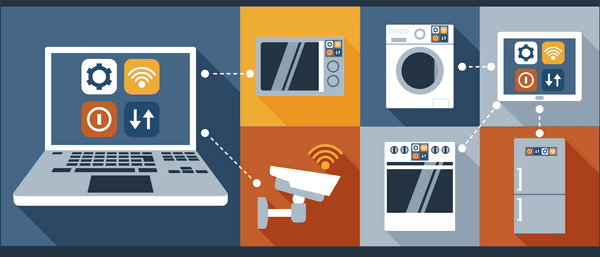
\includegraphics[width=0.5\textwidth]{trainingmaterials/project2-iot/internet-of-things2.png}
    
\end{frame}

\begin{frame}{Internet of Things: Ubiquitous Computing}
    \begin{itemize}
        \item Computing devices present everywhere, anytime
        \item Evolution: Context awareness (knowledge about the environment)
    \end{itemize}
    \centering
    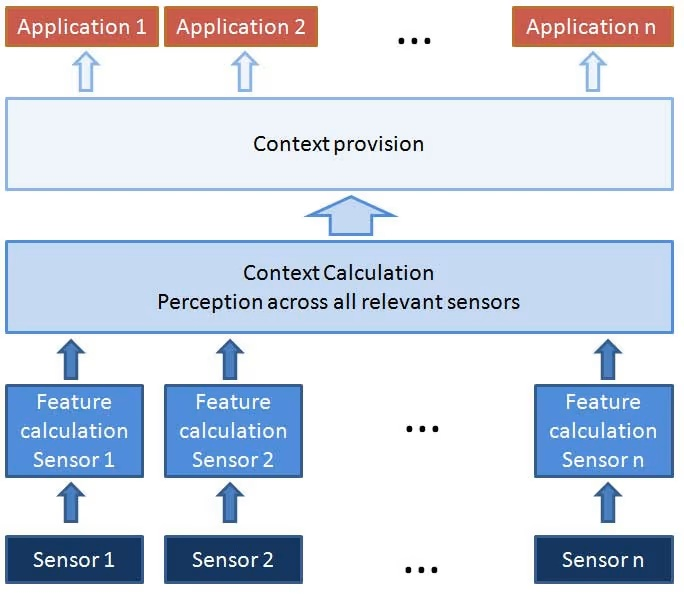
\includegraphics[width=0.5\textwidth]{trainingmaterials/project2-iot/context-aware_computing_systems.jpg}
\end{frame}

\begin{frame}{Internet of Things: Applications}
    \begin{itemize}
        \item Smart Greenhouse
        \begin{itemize}
            \item Plant Health Monitoring
            \item Watering Control
            \item Locate Plants in Greenhouses
            \item Stock and Management
        \end{itemize}
        \begin{center}
             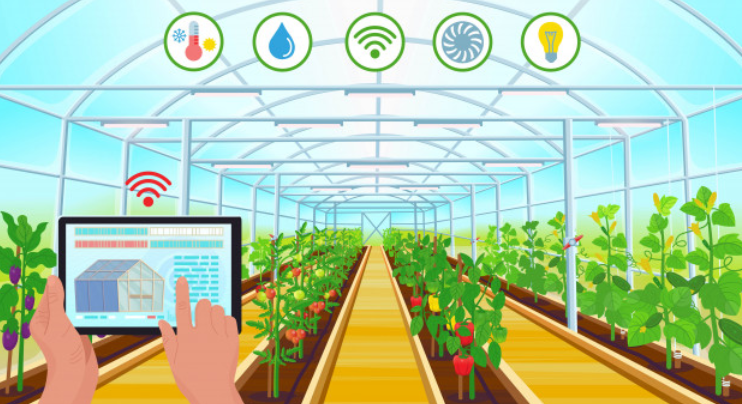
\includegraphics[width=0.5\textwidth]{trainingmaterials/project2-iot/greenhose.png}
        \end{center}
        \item Smart Supermarket
        \begin{itemize}
            \item Automated identification and restocking
            \item Automatic payment authorization
        \end{itemize}
        \item Monitoring elderly/convalescent patients at home
        \item Traffic regulation
        \item Power grid management
    \end{itemize}
\end{frame}

\begin{frame}{Internet of Things: Technologies}
  \begin{itemize}
    \item \textbf{Top Edge/Gateway}
    \begin{itemize}
      \item Linux (67\%)
      \begin{itemize}
        \item Ubuntu (27\%)
        \item Raspbian (28\%)
        \item Debian (28\%)
      \end{itemize}
      \item Windows (26\%)
      \item Android (22\%)
    \end{itemize}
    \item \textbf{Constrained Devices}
    \begin{itemize}
      \item Linux (45\%)
      \item FreeRTOS (29\%)
      \item Bare Metal (21\%)
      \item Zephyr (21\%)
      \item Eclipse Threadx (13\%)
    \end{itemize}
    \item \textbf{Constrained Devices}
    \begin{itemize}
      \item 68\% ARM
      \item 28\% ESP32
      \item 13\% RISC-V
    \end{itemize}
  \end{itemize}

\end{frame}

\begin{frame}{Internet of Things: Technologies}
    \begin{itemize}
        \item Programming Languages 
        \begin{itemize}
            \item Constrained Devices: C (55\%), C++(36\%), Java (29\%), Python(32\%)
            \item Gateways/Edge: Java (32\%), Python(39\%), Javascript (15\%), C++ (29\%)
        \end{itemize}
        \item Connectivity: Cellular (59\%), Ethernet (45\%), WiFi(46\%), Bluetooth (31\%)
        \item Cloud Platforms: AWS(45\%), Azure(22\%), Google Cloud Platform (19\%)
    \end{itemize}
    \footnote{Source: Eclipse IOT Survey 2024 Percentage over complete system of applications under survey. Applications may include more than one technology in the system}
\end{frame}

\section{UDP/IP}
\begin{frame}{UDP/IP}
    \begin{columns}
        \begin{column}{0.5\textwidth}
            \begin{itemize}
                \item System connected on Local Area Network (LAN)
                \item Members: 
                \begin{itemize}
                    \item RPI (Use UDP in Linux)
                    \item Wifi Router
                    \item Host Machine with Virtualized Ubuntu (Use UDP in Linux)
                \end{itemize}
            \end{itemize}
        \end{column}
        \begin{column}{0.5\textwidth}
            \centering
            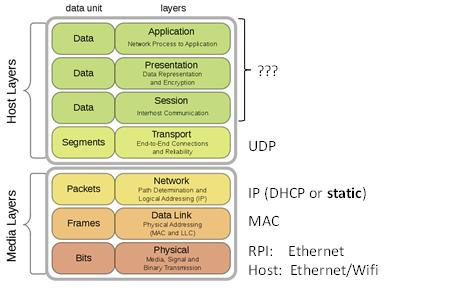
\includegraphics[]{trainingmaterials/project2-iot/ip.jpg}
        \end{column}
    \end{columns}
\end{frame}

\begin{frame}[fragile]{Server UDP/IP  C/C++} % important using minted you need fragile
    \begin{columns}
        \begin{column}{0.35\textwidth}
            \begin{itemize}
                \item UDP Server operation
                    \begin{itemize}
                        \item Create UDP Socket
                        \item Bind Socket to server address (Server IP address)
                        \item Send and receive messages
                        \item Close Socket
                    \end{itemize}
            \end{itemize}  
        \end{column}
        \begin{column}{0.65\textwidth}
            \begin{minted}[fontsize=\scriptsize, bgcolor=blue!5]{c}
    int sockfd = socket(int domain, int type, 
        int protocol);
    
    bind(int sockfd, const struct sockaddr *addr, 
            socklen_t addrlen);
    
    sendto(int sockfd, const void *buf, 
            size_t len, 
            int flags, 
            const struct sockaddr *dest_addr, 
            socklen_t addrlen);
    
    revfrom(int sockfd, const void *buf, 
            size_t len, 
            int flags, 
            const struct sockaddr *dest_addr, 
            socklen_t addrlen);

    close(int sockfd);
    
             \end{minted}      
        \end{column}   
    \end{columns}
\end{frame}

\begin{frame}[fragile]{Client UDP/IP  C/C++} % important using minted you need fragile
    \begin{columns}
        \begin{column}{0.35\textwidth}
            \begin{itemize}
                \item UDP Client operation
                    \begin{itemize}
                        \item Create UDP Socket
                        \item Send and receive messages
                        \item Close Socket
                    \end{itemize}
            \end{itemize}  
        \end{column}
        \begin{column}{0.65\textwidth}
            \begin{minted}[fontsize=\scriptsize, bgcolor=blue!5]{c}
    int sockfd = socket(int domain, int type, 
        int protocol);

    
    sendto(int sockfd, const void *buf, 
            size_t len, 
            int flags, 
            const struct sockaddr *dest_addr, 
            socklen_t addrlen);
    
    revfrom(int sockfd, const void *buf, 
            size_t len, 
            int flags, 
            const struct sockaddr *dest_addr, 
            socklen_t addrlen);

    close(int sockfd);
    
             \end{minted}      
        \end{column}   
    \end{columns}
\end{frame}

\begin{frame}{UDP Client/Server}
\centering
    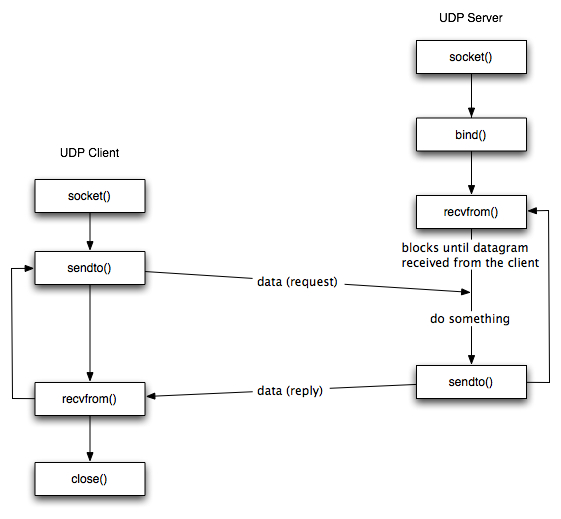
\includegraphics[width=0.65\textwidth]{trainingmaterials/project2-iot/udp-protocol.jpeg}
\end{frame}

\section{Project III: UDP Communication RPI/Ubuntu}
\begin{frame}{System Minimal Requirements (Phase I: Mandatory)}
    \begin{itemize}
        \item Maximun grade 8.5 in 10
            \begin{itemize}
                \item Hard-coding parameters is not allowed
                \item Pay attention to code clarity
            \end{itemize}
        \item Buildroot Linux Project II
        \item UDP Client implemented in RPI
        \item RPI samples data at 1 Sample/s
        \item RPI sends data to server every 10s
        \item Server calculates Mean/Max/Min/Std each minute
        \item Information displayed in server terminal
         \item Sensors: Accelerometer MPU6050 and TCS34725 (RGB)
    \end{itemize}
\end{frame}

\begin{frame}[fragile]{System Minimal Requirements (Phase II: Optional)}
    \begin{itemize} 
        \item 1.5 additional mark 
        \item Remote communications: MQTT Client in RPI (mosquitto client). Use Buildroot software packages
        \item Information display: Thingsboard (dashboard)
            \begin{itemize}
                \item \href {https://thingsboard.io/docs/user-guide/install/ubuntu/}{Thingsboard installation }
                \item You can use the mosquito client installed with Buildroot
                \begin{minted}{bash}
mosquitto_pub -d -q 1 -h “hostip" -p "1883" -t "v1/devices/me/telemetry" -u “xxxxx" -m {“your variable":25}
                \end{minted}
                \item \href{https://thingsboard.io/docs/getting-started-guides/helloworld/?connectdevice=mqtt-linux}{MQTT ...more details}

            \end{itemize}
    \end{itemize}
\end{frame}

\section{Project III Deliverables}
\begin{frame}{Deliverables}
    \begin{itemize}
        \item Source code (Phase I): Both Client/Server side (Commented)
        \item Optional part (in case you complete it)
        \item Due date: 19/05/2025 (8:30)
        \item PowerPoint presentation 
        \item Oral presentation + Demo Class on 19/05/2025 at 12:30
    \end{itemize}
\end{frame}
